\cleardoublepage
\newpage
\ThisULCornerWallPaper{1.0}{chapterimage.eps}
\chapter*{Introdución} % 
\addcontentsline{toc}{chapter}{Introdución} %% Agregando manualmente a la tabla de contenidos

%% Usei a mesma estrutura do inicio do quijote
En mi querido pueblo de Occo, allá en la época de mi primera década, yo pasaba mis días dividiendo mi tiempo entre los trabajos de la chacra\footnote{También escrita como chakra, esta es una palabra quechua que hace referencia a um terreno de cultivo.}, mis juegos infantiles e innumerables paseos por la sierra.
Los trabajos del campo, aunque eran pesados para mí, eran posibles de llevar, pues estos eran divididos con toda la familia. 
Aun así, los días en la sierra no transcurrían limpios de sorpresas, dado que, de cuando en cuando alguno de nuestros animales se extraviaba; en esos casos, nosotros salíamos por las laderas de los montes gritando su nombre hasta que escuchábamos una respuesta, generalmente en forma de un lamento lleno de tristeza y añoranza.
Esta táctica era especialmente eficaz con mi burrito, pues el conseguía escuchar mi llamado desde otras montañas. Así, cuando yo gritaba su nombre, el volvía a mí, gritando y llorando, escogiendo su camino en función de la dirección de mi voz.  
En otras ocasiones percibíamos que desaparecían animales pequeños como pollos o cuyes; sin embargo, después de observar las evidencias y hacer un trabajo detectivesco, descubríamos que su ausencia era debido a la visita de algún halcón, zorro, o gato de montaña.
En esos casos, solo podíamos llorar por ellos; sin embargo, eran pocas las veces que perdíamos animales de esa forma, dado que además de las personas de la casa, nosotros teníamos animales como perros y gatos que nos ayudaban a vigilar.

\begin{wrapfigure}{r}{0.49\textwidth}
  \begin{center}
  \vspace{-20pt}
    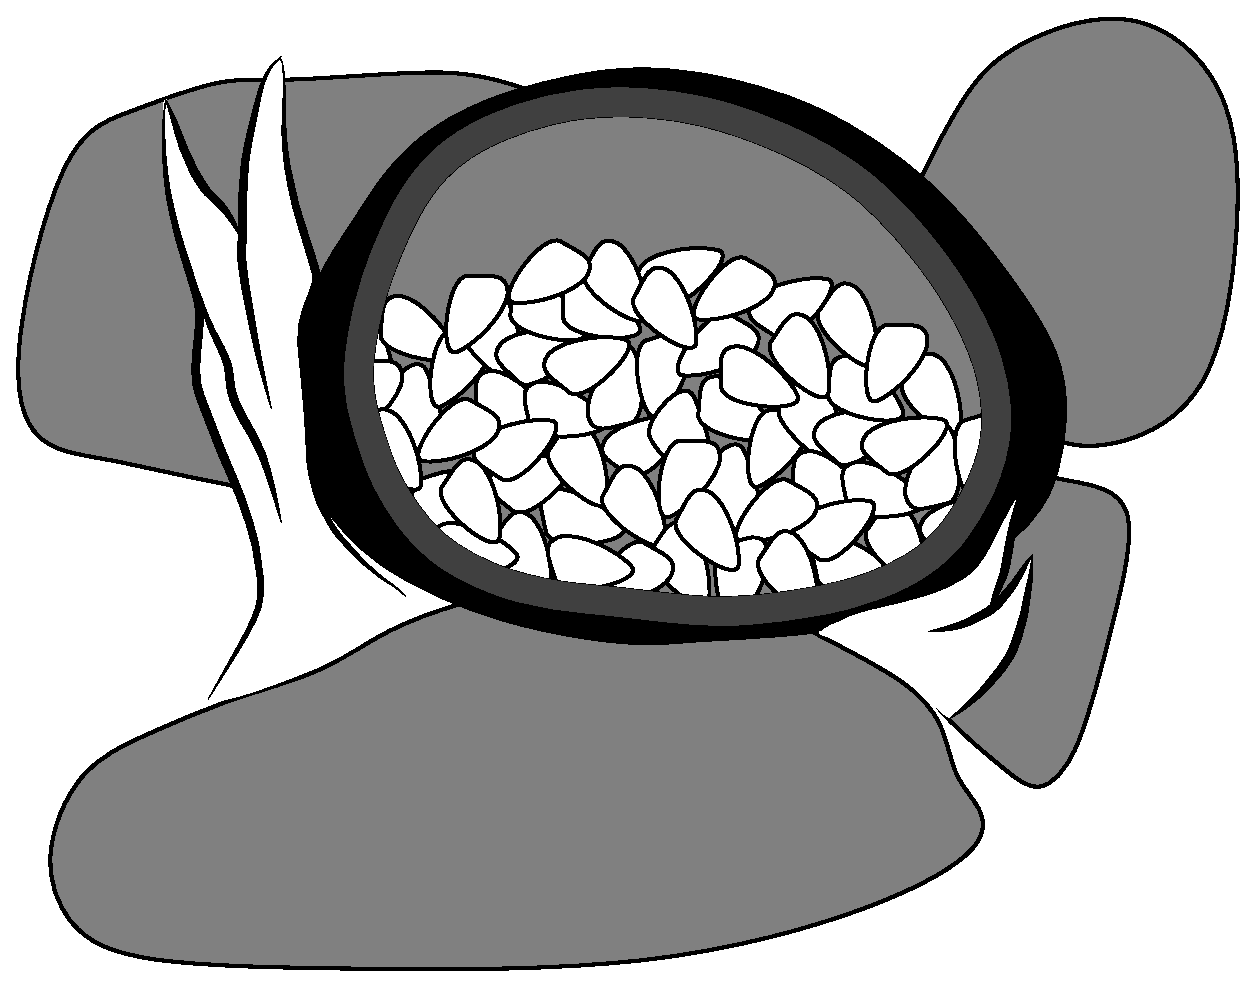
\includegraphics[width=0.47\textwidth]{cancha.eps}
  \end{center}
  \vspace{-20pt}
  %\caption{Zandor}
\end{wrapfigure}
Mi familia no era acomodada, y tal vez ese concepto escapaba a mi comprensión en aquella época, mas nada de lo que realmente me importaba me faltaba.   
Yo recuerdo que mi casa era de adobe y madera, con techo de tejas; mi mamá cocinaba sobre una pequeña fogata, y mis hermanas y yo, ciertamente, usábamos con mucha frecuencia ropa que a simple vista cualquier persona consideraría que eran varias medidas menores de las que necesitábamos;
sin embargo, para mí, mi casa era un castillo amplio y fresco, al cual yo iba a descansar después de volver de la escuela o del trabajo en la chacra.
La cocina de mi mamá era la mejor, ella estaba llena de sabores obtenidos de los mismos productos que cultivábamos o cuidábamos; en días especiales mi papá iba al río y comíamos pescado. Otras veces, en época de sequía, comíamos charqui\footnote{Carne deshidratada al sol.}, con alguna mezcla de huevos de perdiz o de gallina, dependiendo de la suerte del día.
En nuestras comidas no podían faltar el queso y la leche: que tanto podían ser de cabra o de vaca.
Los postres dependían de la estación del año, pues las frutas como tunas, duraznos, higos, pepinos dulces, sanky\footnote{Fruta del Ande peruano que tiene múltiples beneficios para la salud.} entre otras frutas tenían cada una su temporada. También habían épocas para sobremesas elaboradas con maíz fresco y otras con calabaza; con esta última, mi mamá hacía mi mazamorra favorita. Era increíble para mí que: una crema de semejante majestad podía ser construida con un poco de azúcar, canela, clavo de olor y calabaza.

A mis hermanas y a mí nos gustaba jugar juntos, salir a pasear buscando frutas, e ir a apreciar animales silvestres. En general nosotros no teníamos discusiones importantes, sin embargo, debo reconocer que: yo de cuando en cuando acostumbraba hacer alguna maldad.
En esos casos, ellas recurrían a las máximas autoridades de la casa, con los señores que gobernaban y decidían sobre el bien y el mal, es decir: mis padres. 
recuerdo que, al principio, mi papá me hablaba con frases como -- Aurelio, no debes esconder la muñeca de tu hermana, --- si el asunto era más grave el me decía --- ¡Aule! ¿Por qué colocaste un grillo en la cabeza de tu hermana? --- Si mi insistencia en la búsqueda de problemas llegaba a niveles peligrosos para mi existencia, mi papá me decía --- ¡Aulicha! ¿Por qué colocaste ají en el caramelo de tu hermana? ---
Así, cuando yo escuchaba que mi papá me llamaba Aulicha, yo ya sabía que mi suerte había sido decidida y que una chicoteada estaba próxima. La idea de huir siempre pasaba por mi cabeza, pero mis experiencias anteriores me indicaban que eso solamente iba a perjudicarme más, e iba resignado delante de mi papá. Inclusive, en varias ocasiones, el me pedía que lleve ese chicote de tres puntas, pequeño y veloz, que era al mismo tiempo un viejo conocido y mi principal antagonista. 

Mi vida en el campo siempre estaba llena de contrapuntos, tantos eran los momentos tristes como los alegres, y  algunas veces, mas de las que me permitirían pensar que era solo una casualidad, los momentos tristes preparaban un camino inevitable e irreversible a épocas alegres, y viceversa; como un ciclo que se retro-alimenta para mantenerse perpetuo.
Así, una de mi mayores alegrías era cuando mi papá retornaba de viaje, generalmente de la costa del Perú, no solo debido a la tristeza y la añoranza que dejaba su partida y la alegría que traía su retorno, sino también porque el volvía lleno de regalos. 
El nos traía dulces, galletas, juguetes, ropas y artículos diversos; los cuales, comúnmente, nosotros en los Andes no teníamos acceso.
Por otro lado, entre mis momentos mas tristes, estaba la perdida de algún ser querido y la consecuente impotencia al no ser capaz de evitar su partida.
No obstante, todo eso es parte de la vida y me gustaría compartir con ustedes algunos de esos momentos.





%Ayacucho é uma cidade do distrito de Ayacucho, na província de Huamanga, no departamento de Ayacucho, no Peru
